\documentclass{article}

\usepackage{graphicx}
\usepackage{tikz}
\usepackage{tikzsymbols}
\usetikzlibrary{calc,patterns,shapes.geometric}
\pagestyle{empty}
\usepackage[margin=0pt]{geometry}
\geometry{papersize={14in,12in}}

\def\centerarc[#1](#2)(#3:#4:#5){\draw[#1] ($(#2)+({#5*cos(#3)},{#5*sin(#3)})$) arc (#3:#4:#5);}

\begin{document}
	\begin{figure}
		\centering
		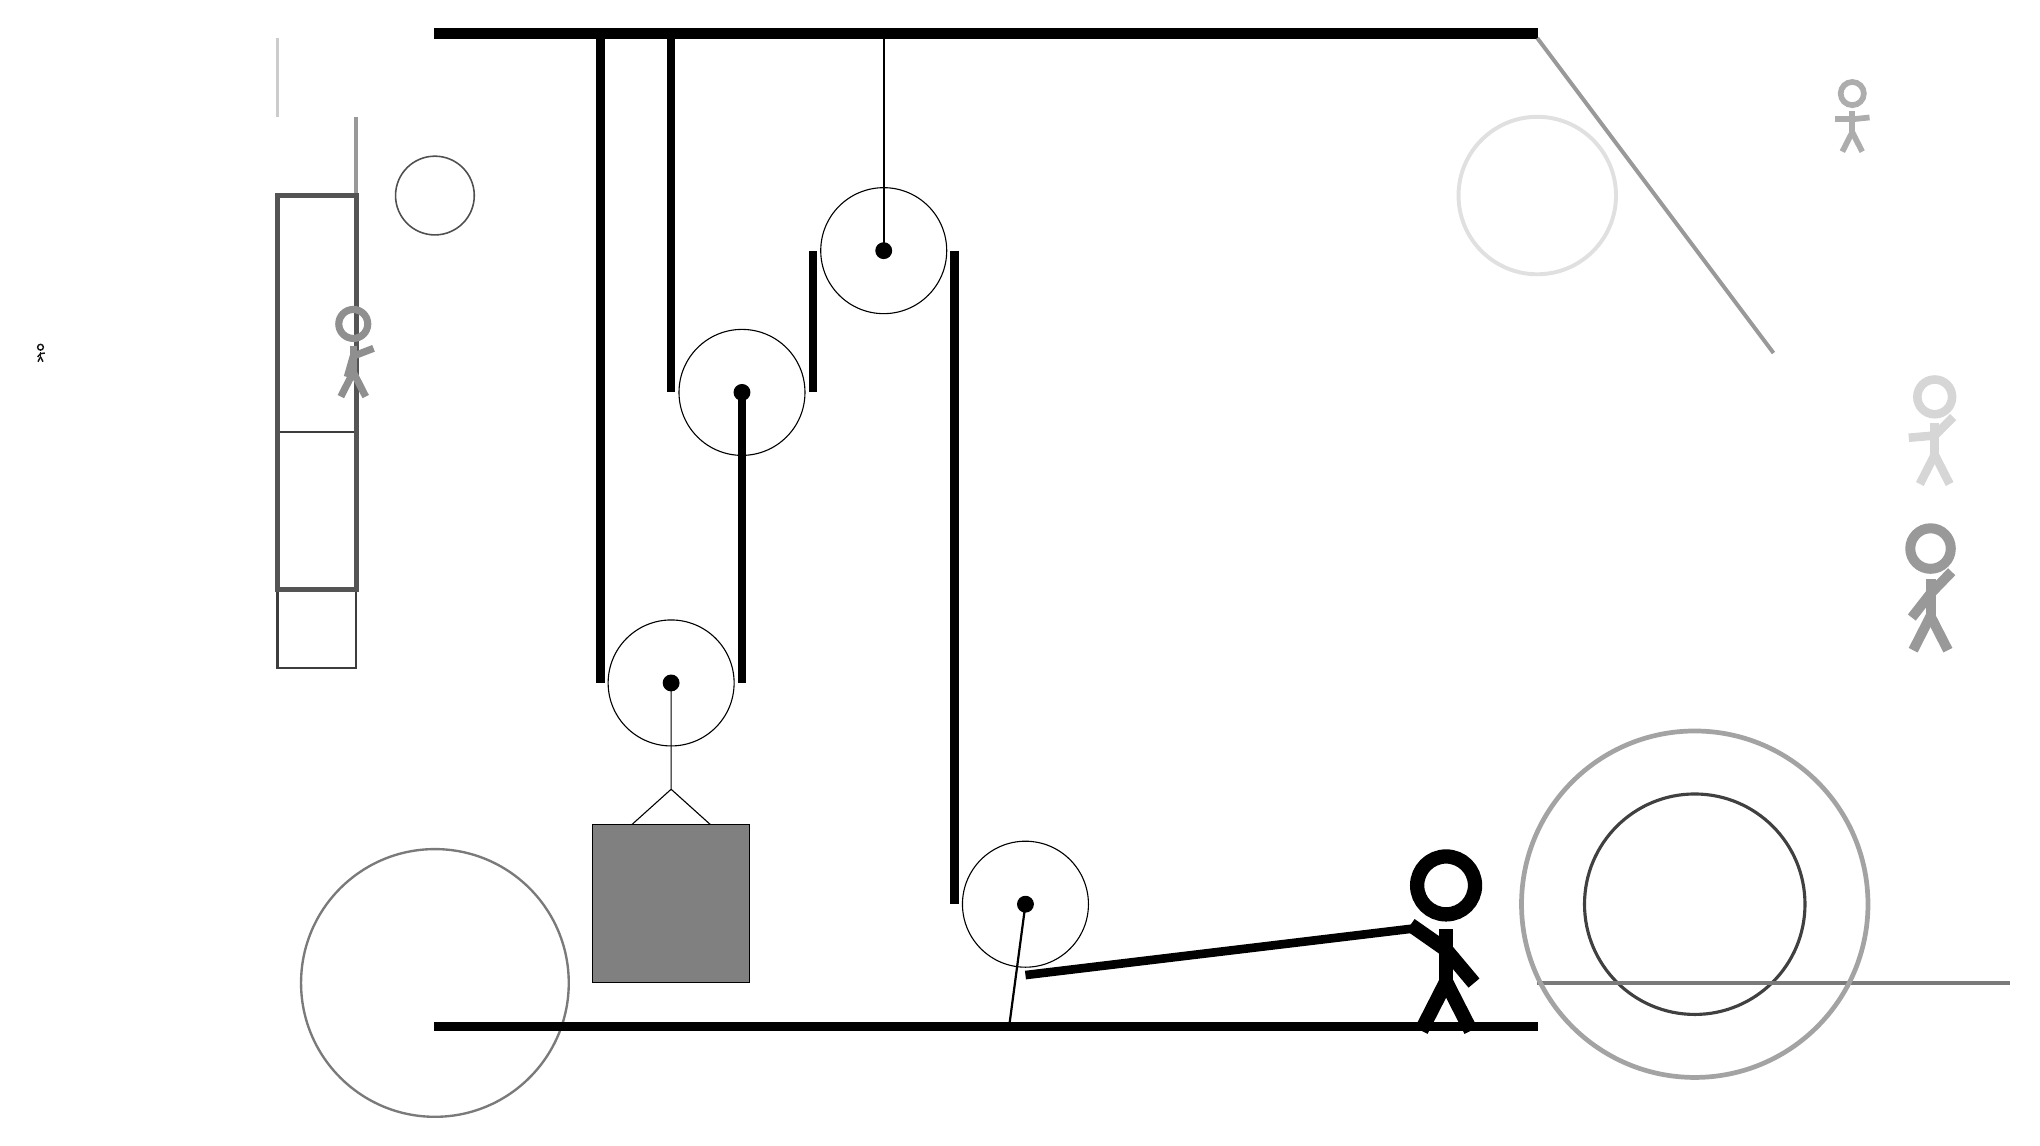
\begin{tikzpicture}
			%%%%% START %%%%%
			
			\draw[fill=black] (-2, 9) rectangle (12, 9.125);
			
			\draw (1, 0.81) circle (0.8);
			\draw[fill=black] (1, 0.81) circle (0.1);
			
			\draw (1.9, 4.5) circle (0.8);
			\draw[fill=black] (1.9, 4.5) circle (0.1);
			
			\draw (3.7, 6.3) circle (0.8);
			\draw[fill=black] (3.7, 6.3) circle (0.1);
			\draw[thick] (3.7, 6.3) -- (3.7, 9);
			
			\draw (5.5, -2) circle (0.8);
			\draw[fill=black] (5.5, -2) circle (0.1);
			\draw[thick] (5.5, -2) -- (5.3, -3.5);
			
			\draw [line width=0.3mm, color=black!52](-2, -3) circle (1.7);
			
			\node[line width=0.7mm, color=black!40] at (17, 2) {\Strichmaxerl[7][52][46]};
			\draw[line width=0.5mm, color=black!40](-3, 8) -- (-3, 3);
			\draw [line width=0.4mm, color=black!75](14, -2) circle (1.4);
			\draw[line width=0.3mm, color=black!76] (-4, 1) rectangle (-3, 4);
			
			\draw[line width=0.5mm, color=black!52](12, -3) -- (18, -3);
			
			\node[line width=0.5mm, color=black!92] at (-7, 5) {\Strichmaxerl[1][49][8]};
			
			\draw[line width=0.3mm, color=black!69] (-2, 9) rectangle (-2, 9);
			\node[line width=0.5mm, color=black!16] at (17, 4) {\Strichmaxerl[6][5][45]};
			
			\node[line width=0.7mm, color=black!32] at (16, 8) {\Strichmaxerl[4][0][6]};
			\draw[line width=0.6mm, color=black!67] (-4, 2) rectangle (-3, 7);
			\node[line width=0.4mm, color=black!44] at (-3, 5) {\Strichmaxerl[5][74][21]};
			\draw [line width=0.5mm, color=black!12](12, 7) circle (1.0);
			\draw[line width=0.5mm, color=black!40](12, 9) -- (15, 5);
			\draw [line width=0.6mm, color=black!36](14, -2) circle (2.2);
			\draw [line width=0.2mm, color=black!69](-2, 7) circle (0.5);
			
			\draw[line width=0.3mm, color=black!20] (-4, 8) rectangle (-4, 9);
			
			\draw (1, 0.81) -- (1, -0.54) -- (0.5, -0.99) -- (1.5, -0.99) -- (1, -0.54);
			\draw[fill=black!50] (0, -0.99) rectangle (2, -2.99);
			\draw[line width=1.1mm] (0.1, 9) -- (0.1, 0.81);
			\centerarc[line width=1.1mm](1, 0.81)(180:360:0.9);
			\draw[line width=1.1mm](1.9, 0.81) -- (1.9, 4.5);
			\draw[line width=1.1mm] (1.0, 9) -- (1.0, 4.5);
			\centerarc[line width=1.1mm](1.9, 4.5)(180:360:0.9);
			\draw[line width=1.1mm](2.8, 4.5) -- (2.8, 6.3);
			\centerarc[line width=1.1mm](3.7, 6.3)(0:180:0.9);
			\draw[line width=1.1mm] (4.6, 6.3) -- (4.6, -2);
			\centerarc[line width=1.1mm](5.5, -2)(0:90:-0.9);
			\draw[line width=1.1mm](5.5, -2.9) -- (10.5, -2.3);
			
			\node at (10.8, -2.5) {\Strichmaxerl[10][-35][-50]};
			
			\draw[fill=black] (-2, -3.5) rectangle (12, -3.6);
			
			%%%%% END %%%%%
		\end{tikzpicture}
	\end{figure}	
\end{document}